%%%%%%%%%%%%%%%%%%%%%%%%%%%%%%%%%%%%%%%%%%%%%%%%%
\section[Selection]{Selection}
%------------------------------------------------
\subsection{Points d'intérêts}
%++++++++++++++++++++++++++++++++++++++++++++++++
\begin{frame}{Points d'intérêts}
  \centering
  \note{
  La première étape consiste à repérer des points d'intérêts sur l'image. Par exemple ici, sur un cube. 
}
  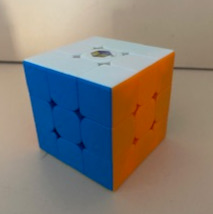
\includegraphics[width=0.6\textwidth]{capture/rub.jpg}
\end{frame}

\begin{frame}{Points d'intérêts}
\note{
Pour un objet convexe tel qu'un cube, il nous suffit de répérer ces sommets pour le reconstruir en 3D.
Mais si l’objet est non convexe, comme dans le schéma de droite, on peut détecter des coins qui ne sont pas représentatifs de la structure globale.
On voit ici que l’enveloppe convexe (en bleu) ne correspond pas exactement à la forme réelle. Ce genre de situation peut gêner certaines étapes de reconstruction.
}
\begin{minipage}[t]{0.48\textwidth}
\centering
\textbf{Points d'intérêts  sur un cube}\\[0.5em]
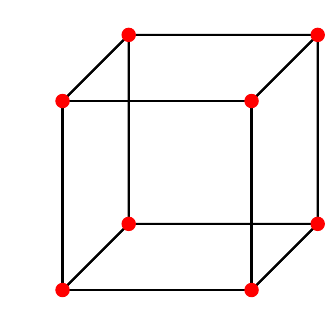
\begin{tikzpicture}[scale=1.2]

% Cube en perspective
\coordinate (A) at (0,0);
\coordinate (B) at (2,0);
\coordinate (C) at (2,2);
\coordinate (D) at (0,2);
\coordinate (E) at (0.7,0.7);
\coordinate (F) at (2.7,0.7);
\coordinate (G) at (2.7,2.7);
\coordinate (H) at (0.7,2.7);

% Faces du cube
\draw[thick] (A) -- (B) -- (C) -- (D) -- cycle; % face avant
\draw[thick] (A) -- (E) -- (F) -- (B); % face basse
\draw[thick] (B) -- (F) -- (G) -- (C);
\draw[thick] (C) -- (G) -- (H) -- (D);
\draw[thick] (D) -- (H) -- (E) -- (A);

\pause
% Coins détectés
\foreach \pt in {(A), (B), (C), (D), (E), (F), (G), (H)} {
  \filldraw[red] \pt circle (2pt);
}

\end{tikzpicture}
\end{minipage}
\hfill
\begin{minipage}[t]{0.48\textwidth}
\centering
\only<2->{
\pause
\textbf{Problème si non convexe}\\[0.5em]
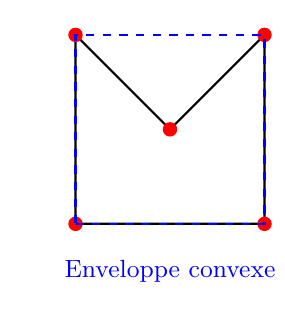
\begin{tikzpicture}[scale=1.2]
% Objet non convexe
\draw[thick] (0,0) -- (2,0) -- (2,2) -- (1,1) -- (0,2) -- cycle;

\pause
% Coins détectés
\foreach \pt in {(0,0), (2,0), (2,2), (1,1), (0,2)} {
  \filldraw[red] \pt circle (2pt);
}

\pause
% Enveloppe convexe
\draw[blue, dashed, thick] (0,0) -- (2,0) -- (2,2) -- (0,2) -- cycle;
\node[blue] at (1,-0.5) {\small Enveloppe convexe};
\end{tikzpicture}
}
\end{minipage}

\end{frame}

\subsection{Algorithme}
%------------------------------------------------

\begin{frame}
  \label{algo-moravec}
\note{
L’algorithme de Moravec est un détecteur de coins assez simple basé sur la variation locale de l’intensité.
Pour chaque pixel, on mesure la variance de l’intensité dans plusieurs directions.
Si la plus petite variance dépasse un certain seuil, on considère qu’on est probablement sur un coin — une zone où l’image change dans toutes les directions.
}
  \hyperlink{moravec-appendix}{
    \beamerbutton{Exemple}
  }
  \hyperlink{moravec-code}{
    \beamerbutton{code}
  }
	\small
\begin{algorithm}[H]
    \caption{\textsf{Moravec (minimum des variances)}}

    \only<1->{\KwIn{Image d’intensité \texttt{image}}}
    \only<2->{\KwOut{Matrice des coins détecté}}
    \only<3->{\BlankLine}
    \only<4->{\ForEach{pixel $(x, y)$ dans l’image}{%
        \only<5->{\Indp$scores \gets$ liste vide\;}}
        \only<6->{\ForEach{direction $(dx, dy)$ parmi : verticale, horizontale, diagonales}{%
            \only<7->{\Indp Calculer la variance locale autour de $(x, y)$ dans la direction $(dx, dy)$\;
            Ajouter la variance à $scores$\;}
        \Indm}
        }
        \only<8->{$score \gets \min(scores)$\;}
        \only<9->{\If{$score >$ \texttt{SEUIL}}{%
            \only<10->{\Indp Marquer $(x, y)$ comme coin\;}
        \Indm}
        }
    \Indm}
    \only<11->{\KwRet{Liste des points marqués}}
\end{algorithm}

\end{frame}

\subsection{Implémentation}

\begin{frame}{Fichier de sortie PBM}
  \note{"Une fois les coins détectés, on peut produire un fichier PBM, ici représenté à droite sous forme de matrice binaire.

Un ‘1’ correspond à un coin détecté. C’est ce fichier qui pourra être ensuite utilisé dans la suite du pipeline, notamment pour l’appariement."}
\begin{minipage}[c]{0.45\textwidth}
  \centering
  \begin{tikzpicture}
    \node[inner sep=0pt] (img) at (0,0) {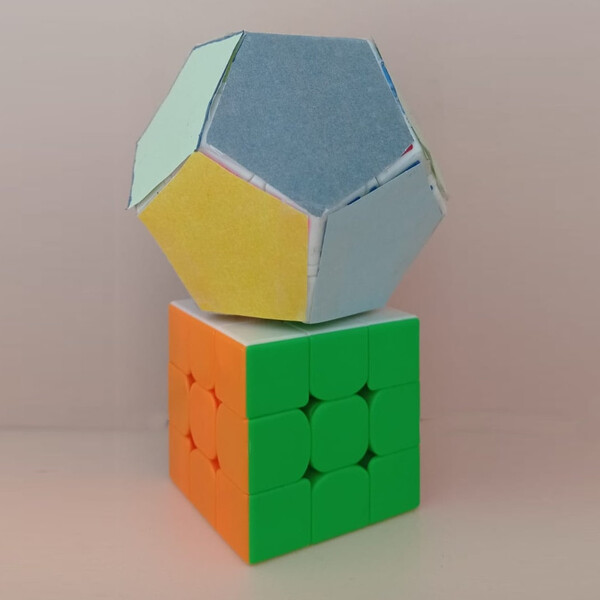
\includegraphics[width=0.9\textwidth]{capture/dodecf0.jpg}};
    \node at (3.5,0) {\Huge$\Rightarrow$};
  \end{tikzpicture}
\end{minipage}
\hfill
\begin{minipage}[c]{0.48\textwidth}
  \centering
  \renewcommand{\arraystretch}{1.2}
  \begin{tabular}{cccccc}
  0 & 0 & 0 & 0 & 0 & 0 \\
  0 & 1 & 1 & 0 & 0 & 0 \\
  0 & 1 & 0 & 1 & 1 & 0 \\
  0 & 0 & 1 & 0 & 0 & 0 \\
  0 & 0 & 1 & 1 & 0 & 0 \\
  0 & 0 & 0 & 1 & 1 & 0 \\
  0 & 1 & 1 & 0 & 0 & 1 \\
  0 & 1 & 0 & 1 & 1 & 0 \\
  0 & 0 & 1 & 0 & 0 & 0 \\
  0 & 0 & 1 & 1 & 0 & 0 \\
  \end{tabular}
\end{minipage}
\end{frame}

\begin{frame}{Influence des paramètres de Moravec}
\note{"Voici quelques exemples de détection de coins selon différents paramètres.

On voit que si on change la taille de la fenêtre ou le seuil, le résultat est très différent.

Avec une fenêtre plus grande, on est plus tolérant au bruit mais on perd en précision.

Et avec un seuil plus faible, on détecte beaucoup plus de coins, parfois à tort.

Il est donc crucial d’ajuster ces paramètres selon les images qu’on traite."}
\begin{minipage}[c]{0.45\textwidth}
\raggedright
\small
\vspace*{\fill}

\textbf{Paramètres utilisés :}
\vspace{1em}

\begin{itemize}
  \setlength\itemsep{0.3em}
  \setlength\leftskip{1em}
  \only<1>{\item \textbf{THRESHOLD} = 2000 \\ \item \textbf{WINDOW} = 4}
  \only<2>{\item \textbf{THRESHOLD} = 2000 \\ \item \textbf{WINDOW} = 6}
  \only<3>{\item \textbf{THRESHOLD} = 4000 \\ \item \textbf{WINDOW} = 10}
  \only<4>{\item \textbf{THRESHOLD} = 500 \\ \item \textbf{WINDOW} = 2}
\end{itemize}

\vspace*{\fill}
\end{minipage}
\hfill
\begin{minipage}[c]{0.48\textwidth}
\centering
\begin{overlayarea}{0.9\linewidth}{4cm}

\only<1>{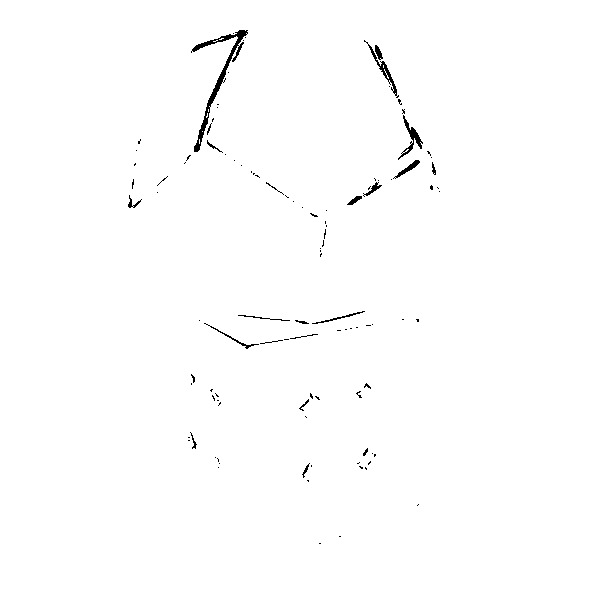
\includegraphics[width=0.9\textwidth]{capture/dodecf0-mv-2000-4-1.jpg}}
\only<2>{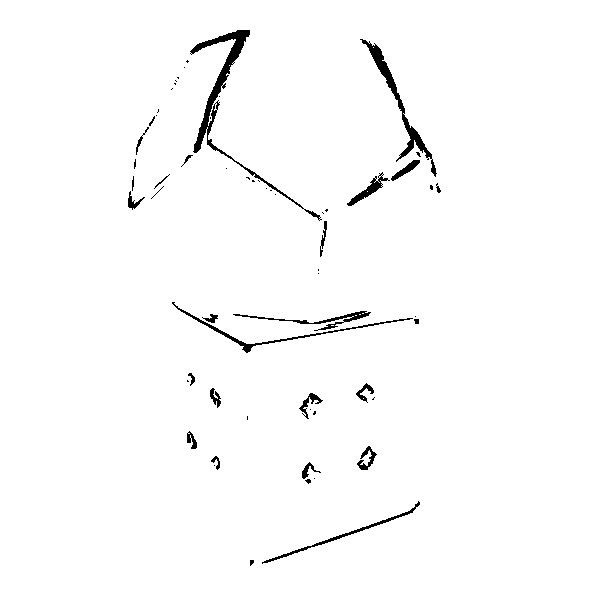
\includegraphics[width=0.9\textwidth]{capture/dodecf0-mv-2000-6-1.jpg}}
\only<3>{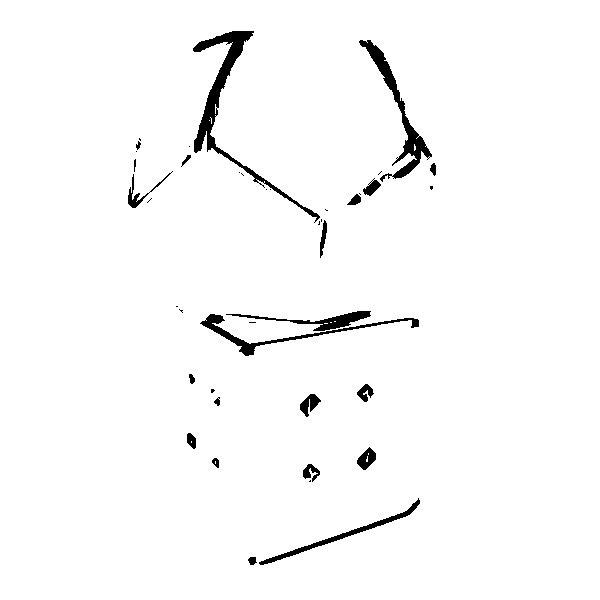
\includegraphics[width=0.9\textwidth]{capture/dodecf0-mv-4000-10-1.jpg}}
\only<4>{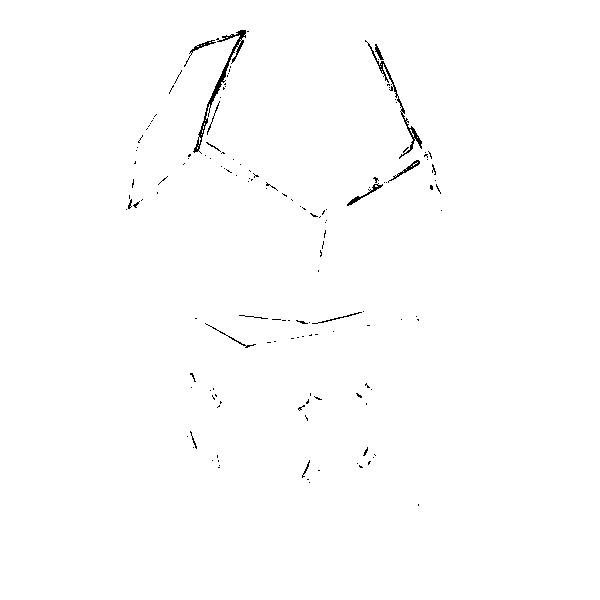
\includegraphics[width=0.9\textwidth]{capture/dodecf0-mv-500-2-1.jpg}}

\end{overlayarea}
\end{minipage}

\end{frame}
